% sec_fss.tex -- textbook v2, Chapter 3: finite-size scaling, done carefully.
% Numbers: facts_fss.md (each with the command that printed it). Rust: rusty-SUNDIALS commit 3eba703 on
% physics/jellium-wigner-2026-10-11. Python: code/fss_disk.py.

\section{Finite-size scaling, done carefully}\label{fss:sec}

A reader of version~1 of this book proposed a natural experiment: \emph{run the Rust crate at $N=72$, $288$ and
$1152$, plot the energy per particle against $1/N$, and extrapolate to $N=\infty$; the finite arrays are \tierX, the
infinite limit is what the theorem is about.} This is a common first idea, and the instinct behind it is sound:
a simulation is finite, the theorem is about an infinite limit, so one should look at how numbers change with size.
The plan needs care in three places, and working out why is a good exercise in what numerics can and cannot do.
\begin{enumerate}
\item In a \emph{periodic box} the perfect lattice has \emph{no} finite-size effect at all: its energy per particle is
exactly the same for every commensurate box large enough for the code's image rule (Section~\ref{fss:sec:box}).
There is nothing to extrapolate. And the smallest box in the list, $N=72$, is too small for the minimum-image rule of
the Rust code, which then returns a wrong energy, below the lattice value.
\item Upstream's definition does not use boxes. It uses \emph{closed disks} centred at the origin
(Chapter~1, Definition~\ref{def:energy}). There finite-size effects are real, and their leading term is proportional
to $N^{-1/2}$, not $N^{-1}$ (Section~\ref{fss:sec:disk}). A fit in $1/N$ alone gives a biased limit.
\item Whatever the fit, an extrapolated number is \tierX. It never becomes \tierA; only the Lean theorem is
(Section~\ref{fss:sec:tiers}).
\end{enumerate}
Relaxed (defected) states have finite-size effects of a third kind, which do not scale cleanly; they appear here only as
exercises (Exercises~\ref{fss:ex:lattice}--\ref{fss:ex:gauss}).

\subsection{Periodic boxes: the perfect lattice has no finite-size effect}\label{fss:sec:box}

Recall the set-up of Section~\ref{sec:num-model}. The box is $L_x\times L_y$, the potential is the shifted-force
$V_{\rm sf}$ with cutoff $r_c$, and the box energy counts each pair once, $E=\sum_{i<j}V_{\rm sf}(|x_i-x_j|_{\rm mi})$.
The box is \emph{commensurate}: its two periods $(L_x,0)$ and $(0,L_y)$ are vectors of the triangular lattice
$\Lambda$ of spacing $a$, so the periods generate a sublattice $\Lambda_{\rm box}\subset\Lambda$, and the $N$ particles
of the perfect lattice are one representative of each coset of $\Lambda/\Lambda_{\rm box}$ (shifted by a common
vector, which changes no difference $x_i-x_j$). For the crate's \texttt{triangular(nx, ny, a)} this holds whenever
\texttt{ny} is even.

\begin{proposition}\label{fss:prop:box}
Let the box be commensurate and $\min(L_x,L_y)\ge2r_c$. Then the minimum-image energy of the perfect triangular lattice
satisfies
\[
\frac{E}{N}=e_{\rm lat}=\frac12\sum_{v\in\Lambda\setminus\{0\}}V_{\rm sf}(|v|),
\]
the value \eqref{eq:elat}, for every such box. In particular $E/N$ does not depend on $N$.
\end{proposition}
\begin{humanproof}
\tierC{} Fix a pair $i\ne j$ and let $d=(d_x,d_y)$ be its minimum image, so $|d_x|\le L_x/2$ and $|d_y|\le L_y/2$. Any
other image is $d+(mL_x,nL_y)$ with $(m,n)\ne(0,0)$. If $m\ne0$ its first coordinate has modulus
$|d_x+mL_x|\ge L_x-|d_x|\ge L_x/2\ge r_c$; if $n\ne0$ the same holds for the second coordinate. Either way that image
has length $\ge r_c$ and contributes $V_{\rm sf}=0$. So
\[
V_{\rm sf}(|d|)=\sum_{s\in\Lambda_{\rm box}}V_{\rm sf}(|x_i-x_j+s|).
\]
Likewise a particle's own images, $s\in\Lambda_{\rm box}\setminus\{0\}$, have $|s|\ge\min(L_x,L_y)\ge2r_c$ and contribute
nothing. Hence
\[
E=\sum_{i<j}V_{\rm sf}(|x_i-x_j|_{\rm mi})=\frac12\sum_{i=1}^N\ \sum_{\substack{j,\ s\in\Lambda_{\rm box}\\(j,s)\ne(i,0)}}V_{\rm sf}(|x_i-x_j+s|).
\]
For fixed $i$, as $j$ runs over the coset representatives and $s$ over $\Lambda_{\rm box}$, the vector $x_i-x_j+s$ runs
over $\Lambda$ exactly once, and $(j,s)=(i,0)$ gives $0$. So the inner sum is $\sum_{v\in\Lambda\setminus0}V_{\rm sf}(|v|)
=2e_{\rm lat}$ for every $i$, and $E=Ne_{\rm lat}$.
\end{humanproof}

The hypothesis $\min(L_x,L_y)\ge2r_c$ belongs to the minimum-image \emph{code}, not to the physics. The Python companion
of Section~\ref{sec:num-python} sums over all images inside $r_c$, including self-images; for that scheme the same
proof works with no condition on the box, and indeed it printed the correct $0.393533366826$ at $N=72$.

\begin{corollary}[a too-small box gives a fake undercut]\label{fss:cor:small}
\tierC{} If the box is commensurate but $\min(L_x,L_y)<2r_c$ and some periodic image other than the minimum one (or a
self-image) lies inside $r_c$, the minimum-image energy per particle is \emph{strictly below} $e_{\rm lat}$.
\end{corollary}
\begin{humanproof}
$V$ is convex, so it lies above its tangent at $r_c$: $V(r)\ge V(r_c)+(r-r_c)V'(r_c)$, i.e.\ $V_{\rm sf}(r)\ge0$, with
equality only at $r=r_c$ (strict convexity, $V''>0$). The minimum-image sum keeps a subset of the non-negative terms of
the full image sum, which equals $Ne_{\rm lat}$ by the argument above; it drops at least one term with $r<r_c$, which is
positive.
\end{humanproof}

For the Rust code this matters. At $r_c=8$ we need both sides $\ge16$. The production box $16a\times9\sqrt3\,a\approx
17.19\times16.75$ ($N=288$) passes. The $6\times12$ box, $6.447\times11.167$ ($N=72$), does not: run there, the code
would report a configuration \emph{below} $e_{\rm tri}$, which prediction P1 of Section~\ref{sec:num-can} would read as a
violation of the theorem. The first suspect, as that section says, is the code.

\begin{numbox}[: the \texttt{fss-lattice} command (Rust)]
\tierX{} We added a subcommand to \texttt{crates/\allowbreak qf-yukawa-crystal/\allowbreak src/\allowbreak main.rs}
(rusty-SUNDIALS branch \texttt{physics/\allowbreak jellium-\allowbreak wigner-\allowbreak 2026-10-11}, commit
\texttt{3eba703141d92fc5a5568a5c2a28e5edb208d25a}, not yet pushed at the time of writing). It uses only the crate's
existing \texttt{System::energy} (pairs $i<j$, each counted once, minimum image), \texttt{triangular} and the helper
\texttt{e\_tri} (the direct lattice sum \texttt{lattice\_energy}). Quoted verbatim:
\begin{lstlisting}[language={},title={main.rs at 3eba703, lines 607--633}]
        "fss-lattice" => {
            // Finite-size check of the perfect triangular lattice in commensurate periodic boxes.
            // With the minimum image, E/N equals the direct lattice sum e_tri exactly once both box sides are
            // >= 2 rc, whatever N is. The 6 x 12 box (6.45 x 11.17, below 2 rc = 16) is the negative control:
            // there the minimum image misses periodic images inside rc, so E/N must come out wrong (too low).
            println!(
                "kappa nx ny N lx ly sides_ge_2rc e_box_per_particle e_tri_direct_sum e_box_minus_e_tri"
            );
            for kappa in [2.0, 1.0] {
                let e_ref = e_tri(kappa);
                for (nx, ny) in [(6, 12), (16, 18), (32, 36), (48, 54)] {
                    let (lx, ly) = (nx as f64 * a, ny as f64 * a * 3.0_f64.sqrt() / 2.0);
                    let sys = System {
                        kappa,
                        rc: 8.0,
                        geometry: Geometry::Periodic { lx, ly },
                    };
                    let n = nx * ny;
                    let e_box = sys.energy(&triangular(nx, ny, a)) / n as f64;
                    let ok = lx.min(ly) >= 2.0 * sys.rc;
                    println!(
                        "{kappa} {nx} {ny} {n} {lx:.4} {ly:.4} {ok} {e_box:.15e} {e_ref:.15e} {:.3e}",
                        e_box - e_ref
                    );
                }
            }
        }
\end{lstlisting}
Output of \texttt{target/release/yukawa\_crystal fss-lattice <dir>} (0.28~s wall clock):
\begin{lstlisting}[language={},basicstyle=\ttfamily\scriptsize,title={yukawa\_crystal fss-lattice}]
kappa nx ny N lx ly sides_ge_2rc e_box_per_particle e_tri_direct_sum e_box_minus_e_tri
2 6 12 72 6.4474 11.1673 false 3.927326193182643e-1 3.935333668255099e-1 -8.007e-4
2 16 18 288 17.1931 16.7509 true 3.935333668255304e-1 3.935333668255099e-1 2.054e-14
2 32 36 1152 34.3862 33.5018 true 3.935333668252588e-1 3.935333668255099e-1 -2.511e-13
2 48 54 2592 51.5794 50.2527 true 3.935333668256187e-1 3.935333668255099e-1 1.088e-13
1 6 12 72 6.4474 11.1673 false 1.563725839041460e0 1.607609217185270e0 -4.388e-2
1 16 18 288 17.1931 16.7509 true 1.607609217185348e0 1.607609217185270e0 7.794e-14
1 32 36 1152 34.3862 33.5018 true 1.607609217184786e0 1.607609217185270e0 -4.841e-13
1 48 54 2592 51.5794 50.2527 true 1.607609217184156e0 1.607609217185270e0 -1.114e-12
\end{lstlisting}
How to read it:
\begin{itemize}
\item \emph{Positive control} (boxes with both sides $\ge16$): $N=288$, $1152$, $2592$ agree with the direct sum to
$\le1.1\times10^{-12}$, i.e.\ to rounding in sums of up to $3.4\times10^6$ pair terms. A plot of these values against
$1/N$ is a horizontal line; its ``extrapolation'' is the value one started with.
\item \emph{Negative control} ($N=72$): the check fires, with the predicted sign. At $\kappa=2$ the box energy is
$8.0\times10^{-4}$ \emph{below} $e_{\rm tri}$, about a tenth of the square--triangular gap $7.43\times10^{-3}$ of
Table~\ref{tab:num-refs}, and two million times the P1 tolerance $4\times10^{-10}$. At $\kappa=1$ (longer range, more
missed images) it is $4.39\times10^{-2}$ below, more than four times the square--triangular gap $9.54\times10^{-3}$.
\item Including $N=72$ in a $1/N$ plot would have produced a beautiful, perfectly spurious finite-size ``trend''.
\end{itemize}
The crate's unit tests still pass after the change (\texttt{cargo test -q --release -j 2 --offline -p
qf-yukawa-crystal -- --test-threads=2}: \texttt{10 passed; 0 failed}).
\end{numbox}

So in a periodic box, finite-size effects are a property of what the particles \emph{do} (defects, relaxation,
temperature), not of the reference energy. Those effects are real but messy; see Exercise~\ref{fss:ex:relax}.

\subsection{Disks: genuine finite-size effects}\label{fss:sec:disk}

Upstream's energy is different: take the points of $C$ in the closed disk $\overline B(0,R)$, count \emph{ordered}
pairs, divide by the number $N(R)$ of points, and take $\liminf_{R\to\infty}$ (Chapter~1, Definition~\ref{def:energy};
\lean{diskEnergy} and \lean{energy}). For $C=\Lat$ every disk is a finite object we can compute exactly, and the limit
is known: by Proposition~\ref{prop:periodic-limit} it exists and equals the lattice sum. We use the Gaussian
$g(t)=e^{-\pi\alpha t}$ at $\alpha=1$, which is admissible, so the limit is
\[
e_\infty=\sum_{a\in\Lat\setminus0}e^{-\pi|a|^2}=\theta_\Lat(1)-1=0.159595266963928\quad\text{\tierX},
\]
computed to rounding (it agrees with Exercise~\ref{ex:py-theta}). This known answer is what makes the disk a good
\emph{positive control} for finite-size scaling: we can check whether an extrapolation recovers it.

\begin{warnbox}[: the factor $\frac12$]
Upstream (and Chapter~1) count ordered pairs, so $e_\infty=\theta_\Lat(1)-1\approx0.1596$. The box energies of this
chapter count each pair once and would give half of that. Compare only numbers in the same convention.
\end{warnbox}

\paragraph{An exact identity.} Let $D=\Lat\cap\overline B(0,R)$ and $N=N(R)=|D|$. Every lattice point sees the same
infinite sum, $\sum_{y\in\Lat,\,y\ne x}g(|x-y|^2)=e_\infty$. The disk sum at $x\in D$ misses exactly the $y$ outside the
disk. Hence:
\begin{proposition}\label{fss:prop:identity}
\tierC{} With the \emph{boundary deficit} $B(R)=\sum_{x\in D}\sum_{y\in\Lat\setminus D}g(|x-y|^2)$,
\[
e(R)=e_\infty-\frac{B(R)}{N(R)} .
\]
\end{proposition}
\begin{humanproof}
$e(R)N(R)=\sum_{x\in D}\sum_{y\in D,\,y\ne x}g=\sum_{x\in D}\bigl(e_\infty-\sum_{y\notin D}g\bigr)=N(R)e_\infty-B(R)$.
All sums have non-negative terms and converge (Gaussian decay), so the rearrangement is allowed.
\end{humanproof}

\paragraph{The scaling argument.} \tierC{} (a heuristic, not a proof). Only points within a few spacings of the circle
contribute to $B(R)$, because $g$ decays fast. Near a straight piece of boundary with outward normal $n$, a pair
$(x,x+v)$ with $x$ inside and $x+v$ outside occurs when $x$ lies in a strip of width $(v\cdot n)_+$ along the edge;
at density one there are $(v\cdot n)_+$ such $x$ per unit length. Averaging over the directions $n$ met along a circle,
$\langle(v\cdot n)_+\rangle=|v|/\pi$, so the deficit per unit length is
\[
\beta=\frac1\pi\sum_{v\in\Lat\setminus0}g(|v|^2)\,|v| ,\qquad B(R)\approx2\pi R\,\beta .
\]
With $N\approx\pi R^2$, i.e.\ $R\approx\sqrt{N/\pi}$,
\[
e(N)\approx e_\infty+\frac{c}{\sqrt N}+\frac dN+(\text{oscillations}),\qquad c_{\rm pred}=-2\sqrt\pi\,\beta .
\]
The $d/N$ term collects the curvature of the circle (the strip inside a circle has area $2\pi Rw-\pi w^2$, not
$2\pi Rw$). The oscillations have two sources: the points near the circle are not spread evenly (the boundary deficit
fluctuates around $2\pi R\beta$), and the count itself fluctuates. For the count, Lemma~\ref{ch5:lem:count} gives
$|N(R)-\pi R^2|=O(R)$, so $N=\pi R^2(1+O(1/R))$, and the denominator's fluctuation changes $B/N$ only at order
$1/N$. Sharper bounds on the lattice-point error are a famous research topic (the Gauss circle problem); this book
proves only the $O(R)$ of Lemma~\ref{ch5:lem:count} and \emph{measures} the rest.

Why $N^{-1/2}$ and not $N^{-1}$? Because the defect is a boundary effect: the boundary has length $\propto R$, the
bulk has area $\propto R^2$, and $R/R^2=1/R\propto N^{-1/2}$. In a periodic box there is no boundary, which is why the
previous subsection found nothing.

\begin{numbox}[: \texttt{code/fss\_disk.py}]
\tierX{} The script computes $e(R)$ by the definition for 362 distinct closed disks with $4\le R\le130$ ($55\le N\le
53\,071$). Disk membership is decided in integer arithmetic, $Q(j,k)=j^2+jk+k^2\le Q_{\max}$ with
$|p(j,k)|^2=Q/b$ (Lemma~\ref{ch2:lem:norm}), and each radius is placed half-way between two shells, so no point is ever
on the circle. The pair sum uses every offset with $|v|^2\le40$ (120 offsets; the neglected tail is below
$e^{-40\pi}\approx4\times10^{-55}$ per pair). The core:
\lstinputlisting[language=Python,firstline=53,lastline=95,title={code/fss\_disk.py, lines 53--95}]{code/fss_disk.py}
Run as \texttt{taskset -c 6,7 python -I code/fss\_disk.py figures\_v2/fss\_disk.pdf} (12.5~s). Output, abridged
(full output in \texttt{facts\_fss.md}):
\begin{lstlisting}[language={},basicstyle=\ttfamily\tiny,title={fss\_disk.py (abridged)}]
exact limit theta_A(1)-1 = 0.159595266963928   theta_Z2(1)-1 = 0.180340599016096
control brute vs offsets: n=  199  e_offsets=0.145954450343741  e_brute=0.145954450343741  diff=-5.6e-17
control brute vs offsets: n=  793  e_offsets=0.152547797510471  e_brute=0.152547797510471  diff=-5.6e-17
   R        n      e(R)               e(R)-e_inf      (n-pi R^2)/R
   8.22    211  0.146729163409227  -1.286610e-02  -0.1478
  26.79   2245  0.155540998312996  -4.054269e-03  -0.3566
  87.02  23785  0.158339845552686  -1.255421e-03  -0.0759
 130.00  53071  0.158755808502495  -8.394585e-04  -0.1594
max |n - pi R^2|/R over all disks: 1.5266; for R > 60: 0.4676
edge prediction (Tier C): beta = 0.054618,  c_pred = -2 sqrt(pi) beta = -0.193616
 nmin=  100 (347 disks, n up to 53071)
   e_inf + c/sqrt(N) + d/N : e_inf=0.159599494 bias=+4.23e-06 c=-0.19398 d=0.0040  rms resid=1.80e-04
   e_inf + c/sqrt(N)       : e_inf=0.159595622 bias=+3.55e-07 c=-0.19365
   e_inf + d/N  (neg ctrl) : e_inf=0.157066869 bias=-2.53e-03 d=-2.1793
 nmin= 1000 (229 disks, n up to 53071)
   e_inf + c/sqrt(N) + d/N : e_inf=0.159597422 bias=+2.15e-06 c=-0.19398 d=0.0132  rms resid=2.86e-05
   e_inf + d/N  (neg ctrl) : e_inf=0.158334757 bias=-1.26e-03 d=-5.6471
square lattice Z^2, 3-term fit (n >= 100): e_inf=0.180356622  minus theta_Z2-1: +1.60e-05  minus theta_A-1: +2.076e-02
\end{lstlisting}
\end{numbox}

How to read it, step by step.
\begin{enumerate}
\item \emph{Positive control on the code.} The fast offset sum and the $O(N^2)$ definition (float coordinates, all
pairs) agree to $6\times10^{-17}$ on four disks with $N$ from 55 to 793. Only then are the large disks read.
\item \emph{The finite-size effect is real and large.} At $N=53\,071$ the disk energy is still $8.4\times10^{-4}$ below
the limit, eleven orders of magnitude above rounding. It is always below, as Proposition~\ref{fss:prop:identity}
requires ($B\ge0$).
\item \emph{The $N^{-1/2}$ law fits, with the predicted slope.} The three-term fit over $N\ge100$ returns
$e_\infty$ within $4.2\times10^{-6}$ of the exact value and $c=-0.19398$, against the edge prediction
$c_{\rm pred}=-0.19362$ (0.2\% apart). A naive continuum estimate, replacing the lattice sum in $\beta$ by an integral,
would give $\beta=1/(2\pi)$ and $c=-1/\sqrt\pi\approx-0.564$, three times too large: the Gaussian at $\alpha=1$ is narrower
than the lattice spacing, so the discreteness matters.
\item \emph{Accuracy is limited by the oscillations, not by rounding.} The residuals of the three-term fit have rms
$1.8\times10^{-4}$ ($N\ge100$) and $2.9\times10^{-5}$ ($N\ge1000$). They are the lattice-point fluctuations. The fitted
$d$ ($0.0040$ or $0.0132$ depending on the range) is not stable: at this level the $1/N$ term cannot be separated from
the oscillations, and the two-term fit happens to land closer. Report $e_\infty$ to the precision the residuals allow
(about $10^{-5}$ here), not to the digits the fit prints.
\item \emph{The Gauss-circle fluctuation is visible.} $(N(R)-\pi R^2)/R$ stays bounded, at most $1.53$ over all disks
and $0.47$ for $R>60$, as Lemma~\ref{ch5:lem:count} allows (Figure~\ref{fss:fig:disk}, right). That it seems to shrink
is an observation, \tierX; we prove nothing beyond $O(R)$.
\item \emph{Negative control 1, the wrong law.} Fitting $e_\infty+d/N$ alone gives $e_\infty=0.157067$, biased by
$-2.53\times10^{-3}$ (about 600 times the three-term error, and 12\% of the gap $2.07\times10^{-2}$ between the square and
triangular limits). Restricting to $N\ge1000$ halves the bias but does not remove it ($-1.26\times10^{-3}$): a wrong
law gives a bias that drifts with the fit window, which is itself a warning sign.
\item \emph{Negative control 2, the wrong configuration.} The same pipeline on $\Z^2$ extrapolates to $0.180357$,
$1.6\times10^{-5}$ from $\theta_{\Z^2}(1)-1$ and $2.08\times10^{-2}$ above the triangular value. The procedure can tell
the two lattices apart; it is not just returning what we hoped.
\end{enumerate}

\begin{figure}[htbp]\centering
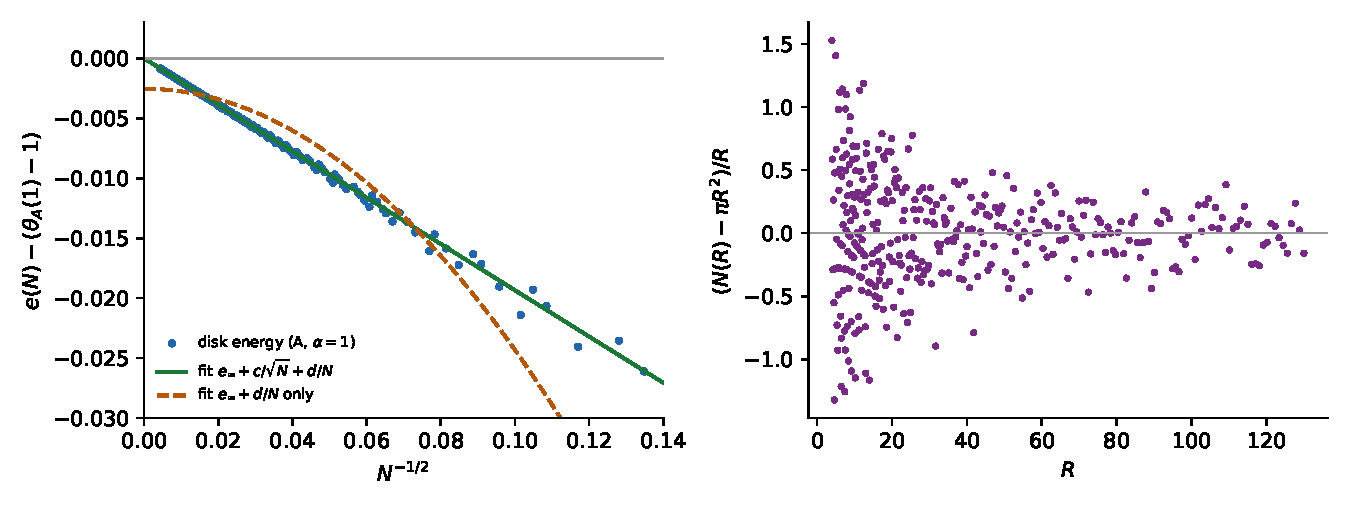
\includegraphics[width=\textwidth]{figures_v2/fss_disk.pdf}
\caption{Finite-size scaling of upstream's closed-disk energy for $\Lat$, Gaussian $\alpha=1$, ordered pairs.
Left: $e(N)-(\theta_\Lat(1)-1)$ against $N^{-1/2}$ (dots), with the fit $e_\infty+c/\sqrt N+d/N$ (solid) and the
pure $1/N$ fit (dashed, a parabola in this variable), both over $N\ge100$; the dashed curve misses the data and the
limit. Right: the lattice-point error $(N(R)-\pi R^2)/R$, radii half-way between shells. Generated by
\texttt{code/fss\_disk.py}. \tierX.}\label{fss:fig:disk}
\end{figure}

\begin{warnbox}[: the $1/N$ trap]
``Plot against $1/N$ and read off the intercept'' is the right recipe only when the correction really is $\propto1/N$
(for example a smooth bulk correction in a periodic system). For an open finite sample the leading correction is the
surface, $\propto N^{-1/2}$ in two dimensions ($N^{-1/3}$ in three). In the variable $1/N$ the data then bend
sharply near the origin, and a straight-line fit through moderate $N$ misses the intercept, here by $2.5\times10^{-3}$.
Before fitting, \emph{derive} the leading correction from the geometry, then check the fitted coefficient against the
derivation (here $c$ against $c_{\rm pred}$), and test the whole pipeline on a case with a known answer.
\end{warnbox}

\subsection{What finite-size scaling can and cannot certify}\label{fss:sec:tiers}

The lesson of Section~\ref{sec:num-can} applies without change.
\begin{itemize}
\item Every number above, including the extrapolated $e_\infty$, is \tierX. An extrapolation is a model fitted to
finitely many floating-point values; with more data or a different window it moves (compare the two fit windows). It
never becomes \tierA.
\item The statement ``the lower energy of $\Lat$ for this $g$ is $\theta_\Lat(1)-1$, and no locally finite density-one
configuration does better'' is \tierA{} only because of the kernel-checked theorem
(\lean{universal_energy_minimum}, conditional on the fidelity of the definitions), and the identification of its
value with the theta series is the Poisson-summation fact of Chapter~1, not the fit.
\item What finite-size scaling \emph{can} do is check consistency: our disk numerics converge, at the rate the geometry
predicts, to the value the theorem names, and they distinguish $\Lat$ from $\Z^2$. If they had not, the first suspects
would be the code, then the fit model, and only last the mathematics. This is the ``theorem as a test oracle'' use of
Section~\ref{sec:num-can}.
\item For periodic boxes there is nothing to extrapolate for the perfect lattice
(Proposition~\ref{fss:prop:box}), and a box too small for the code's image rule produces a spurious ``undercut''
(Corollary~\ref{fss:cor:small}). Check the image condition before reading any energy.
\end{itemize}

\subsection{Exercises on finite-size effects}

\begin{exercise}[Box size and the image rule]\label{fss:ex:lattice}
(a) Using \texttt{yukawa\_crystal fss-lattice}, add the boxes $(nx,ny)=(8,16)$, $(14,16)$ and $(16,16)$ (all commensurate)
and predict, \emph{before} running, which pass $\min(L_x,L_y)\ge2r_c=16$ and the sign of $e_{\rm box}-e_{\rm tri}$ for
each. (b) Prove that at $(16,16)$, where $L_y=8\sqrt3a\approx14.89<16$, some image other than the minimum one lies inside
$r_c$, so Corollary~\ref{fss:cor:small} applies. (c) Replace the minimum image by a loop over image shells as in the
Python companion and show that the $N=72$ row then agrees with $e_{\rm tri}$. Which row is the positive control and which
the negative control after your change?
\end{exercise}

\begin{exercise}[Relaxations at $N=288$ and $N=1152$: a proposal]\label{fss:ex:relax}
On a machine you are allowed to use for hours, repeat the $T=0$ quench study of Section~\ref{sec:num-results} at
$N=288$ ($16\times18$) and $N=1152$ ($32\times36$), $\kappa=2$, from uniform random starts. The crate's \texttt{main}
command reads $N=288$ initial conditions and uses \texttt{tri\_box}, so you must add a variant; preregister the
predictions first and commit them before the code. Measure, per run: the excess energy per particle
$e-e_{\rm tri}$, the defect fraction, and whether the lattice is reached; report the distributions, not only the means.
Then explain why these numbers need not converge cleanly with $N$: the number of local minima grows quickly with $N$,
so ``fraction reaching the lattice'' tends to fall; the excess energy per particle of a state with $k$ defects is
roughly $k\,\epsilon_{\rm def}/N$, and $k$ depends on the quench protocol, not only on $N$; and the cost grows as well
(the dense Hessian is $2N\times2N$, so the Jacobi spectrum costs $4^3=64$ times more at four times $N$). Every result is
\tierX{} and says nothing about the theorem.
\end{exercise}

\begin{exercise}[Plant the factor-two bug]\label{fss:ex:half}
In \texttt{fss\_disk.py} divide the disk energy by $2$ (``count each pair once''), but keep the reference
$\theta_\Lat(1)-1$. Which printed check fires, and by how much? Then also halve the reference: which checks still pass,
and what does that tell you about controls that share a convention with the quantity they check?
\end{exercise}

\begin{exercise}[Measure the lattice-point error]\label{fss:ex:gauss}
Extend the right panel of Figure~\ref{fss:fig:disk} to $R=2000$, counting only (no energies). Fit
$\max_{R'\le R}|N(R')-\pi R'^2|$ to $C R^{\theta}$ on a log--log plot. What $\theta$ do you see? Why is your answer
\tierX{}, and why can no finite computation prove that $\theta<1$? Compare with what Lemma~\ref{ch5:lem:count} proves.
Then repeat the disk-energy fit of this section at $\alpha=2$ and $\alpha=1/2$: how do $\beta$, $c$ and the residual size
change with the width of the Gaussian?
\end{exercise}
